\usetikzlibrary{arrows}
\renewcommand{\familydefault}{\sfdefault}
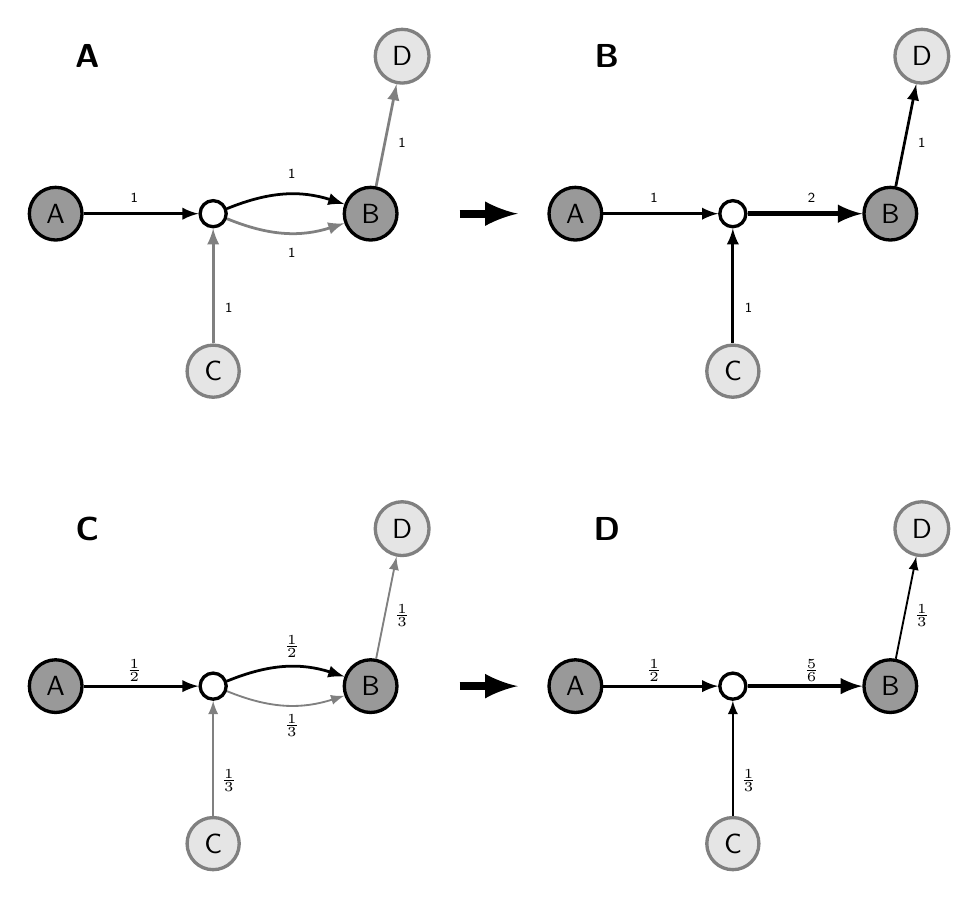
\begin{tikzpicture}[node distance=2cm, auto, thick, scale = 2.0, font=\tiny]
    \tikzstyle{node_black} = [draw=black, very thick, circle, fill=gray!80, shorten <=1pt, shorten >=1pt, font=\sf]
    \tikzstyle{node_gray} = [draw=gray, very thick, circle, fill=gray!20, shorten <=1pt, shorten >=1pt, font=\sf]
    \tikzstyle{node_empty} = [draw=black, very thick, circle, fill=none]
    \tikzstyle{arrow_black} = [->, black, line width=1, >=latex]
    \tikzstyle{arrow_grey} = [->, gray, line width=1, >=latex]

    \node[node_black] (nA) at (0,4.0) {A};
    \node[node_empty] (no) at (1,4.0) {};
    \node[node_gray] (nC) at (1,3.0) {C};
    \node[node_black] (nB) at (2,4.0) {B};
    \node[node_gray] (nD) at (2.2,5.0) {D};

    \draw[arrow_black] (nA) edge  (no);
    \draw[arrow_grey] (no) edge [bend right=20] (nB);
    \draw[arrow_grey] (nC) edge (no);
    \draw[arrow_black] (no) edge [bend left=20] (nB);
    \draw[arrow_grey] (nB) edge (nD);

    \node[draw=none] at (0.5,4.1) {1};
    \node[draw=none] at (1.5,4.25) {1};
    \node[draw=none] at (1.1,3.4) {1};
    \node[draw=none] at (1.5,3.75) {1};
    \node[draw=none] at (2.2,4.45) {1};

    \node[draw=none,font={\large\bf}] at (0.2,5.0) {A};

    % ---------------------------------------

    \node[draw = none] (m1) at (2.5, 4.0) {};
    \node[draw = none] (m2) at (3, 4.0) {};
    \draw[->, black, line width = 3, >=latex]  (m1) edge (m2);

    % ---------------------------------------

    \node[node_black] (nA) at (3.3,4.0) {A};
    \node[node_empty] (no) at (4.3,4.0) {};
    \node[node_gray] (nC) at (4.3,3.0) {C};
    \node[node_black] (nB) at (5.3,4.0) {B};
    \node[node_gray] (nD) at (5.5,5.0) {D};

    % 1/2 = 1; 1/3 = 2/3; 5/6 = 5/3
    \draw[arrow_black, line width=1] (nA) edge  (no);
    \draw[arrow_black, line width=2] (no) edge (nB);
    \draw[arrow_black, line width=1] (nC) edge (no);
    \draw[arrow_black, line width=1] (nB) edge (nD);

    \node[draw=none] at (3.8,4.1) {1};
    \node[draw=none] at (4.8,4.1) {2};
    \node[draw=none] at (4.4,3.4) {1};
    \node[draw=none] at (5.5,4.45) {1};

    \node[draw=none,font={\large\bf}] at (3.5,5.0) {B};

    % ---------------------------------------

    \node[node_black] (nA) at (0,1) {A};
    \node[node_empty] (no) at (1,1) {};
    \node[node_gray] (nC) at (1,0) {C};
    \node[node_black] (nB) at (2,1) {B};
    \node[node_gray] (nD) at (2.2,2) {D};

    \draw[arrow_black] (nA) edge  (no);
    \draw[arrow_grey, line width=2/3] (no) edge [bend right=20] (nB);
    \draw[arrow_grey, line width=2/3] (nC) edge (no);
    \draw[arrow_black] (no) edge [bend left=20] (nB);
    \draw[arrow_grey, line width=2/3] (nB) edge (nD);

    \node[draw=none] at (0.5,1.1) {$\frac{1}{2}$};
    \node[draw=none] at (1.5,1.25) {$\frac{1}{2}$};
    \node[draw=none] at (1.1,0.4) {$\frac{1}{3}$};
    \node[draw=none] at (1.5,0.75) {$\frac{1}{3}$};
    \node[draw=none] at (2.2,1.45) {$\frac{1}{3}$};

    \node[draw=none,font={\large\bf}] at (0.2,2.0) {C};

    % ---------------------------------------

    \node[draw = none] (m1) at (2.5, 1) {};
    \node[draw = none] (m2) at (3, 1) {};
    \draw[->, black, line width = 3, >=latex]  (m1) edge (m2);

    % ---------------------------------------

    \node[node_black] (nA) at (3.3,1) {A};
    \node[node_empty] (no) at (4.3,1) {};
    \node[node_gray] (nC) at (4.3,0) {C};
    \node[node_black] (nB) at (5.3,1) {B};
    \node[node_gray] (nD) at (5.5,2) {D};

    % 1/2 = 1; 1/3 = 2/3; 5/6 = 5/3
    \draw[arrow_black, line width=1] (nA) edge  (no);
    \draw[arrow_black, line width=5/3] (no) edge (nB);
    \draw[arrow_black, line width=2/3] (nC) edge (no);
    \draw[arrow_black, line width=2/3] (nB) edge (nD);

    \node[draw=none] at (3.8,1.1) {$\frac{1}{2}$};
    \node[draw=none] at (4.8,1.1) {$\frac{5}{6}$};
    \node[draw=none] at (4.4,0.4) {$\frac{1}{3}$};
    \node[draw=none] at (5.5,1.45) {$\frac{1}{3}$};

    \node[draw=none,font={\large\bf}] at (3.5,2.0) {D};

\end{tikzpicture}
